\appendix
\renewcommand{\thechapter}{B}
\renewcommand{\chaptername}{Appendix}

\chapter{Implementing steering procedure}


\section{Steering Procedure}

%% Steering approach
This is a description of the horizontal steering method I used to steer the 6 mA beam on November, 2015. The final solution was saved as settings file kiersten\_6mA\_151116.csv.

The procedure for horizontal steering attempts to steer the beam as close as possible to the center of the quads in the first turn, and use two dipoles at the end of the ring to close the orbit. I generated this solution using an existing solution with many turns, but it should be possible to apply this method to a ring with "no-steering" (significant current loss in the first few turns).
The procedure is as follows:

\begin{enumerate}
\item Set last 2 injection dipoles by scanning currents and identifying smallest rms deviation in first two RQ's after injection. Time: 1 hour.
\item Steer through RQ3 (first turn) by setting current in D1; Repeat injection scan if change was significant. Time: 10 minutes + 1 hour if repeating injection scan.
\item Steer through quads in first turn, setting dipoles D2-34 in order and using quad-as-BPM method to measure position in quads. Time: 2 1/2 hours ($\times 2$ for best results).
\item Close orbit by scanning D34 and D35 currents.  Time: 30 minutes
\item Verify orbit quality by running quad scan for 1st turn quad-as-BPM data, and look at multi-turn BPM data to estimate orbit excursions from closed orbit. Time: 30 minutes.
\end{enumerate}

 Total (minimum) time for steering: $\approx 6$ hours. Time estimates are for total measurement/ beam-on time, more time should be added for trouble-shooting and general unruly behavior.
 
 
 
 %todo: UPDATE THIS PLOT!
\begin{figure}[!h]
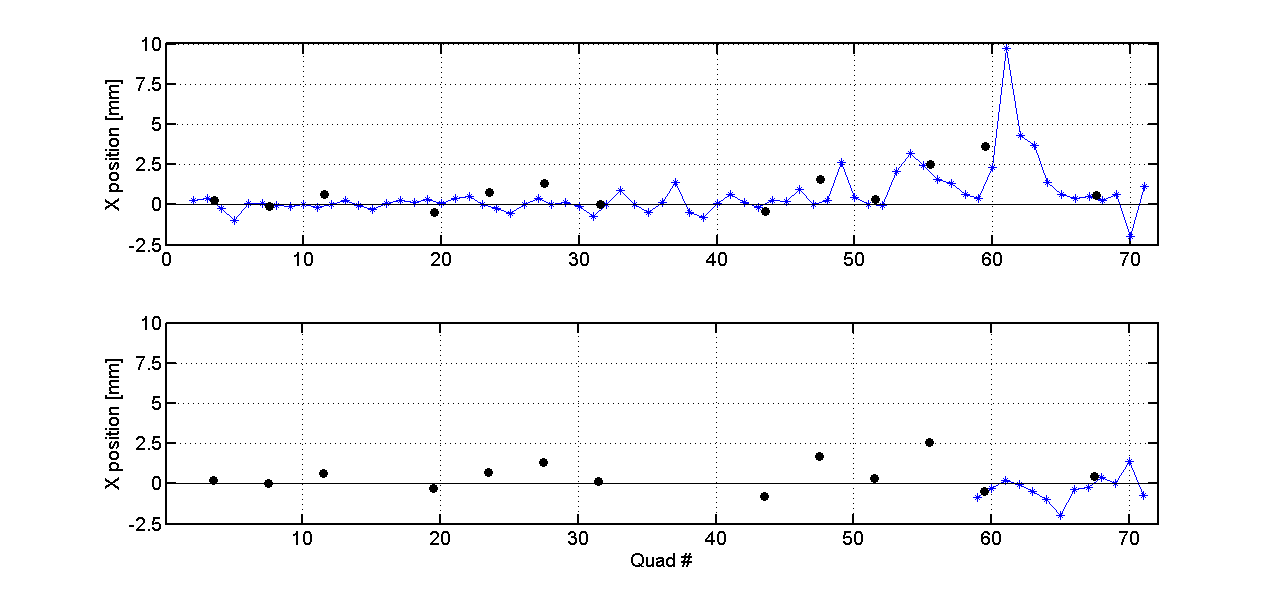
\includegraphics[width=\textwidth]{4.figures/quadscan_151113_151116.png}
\caption{1st turn solution generated on 11/13/15 (top) and 11/16/15 (bottom), by steering through defocusing quadrupoles.}
\label{fig:ring_steering}
\end{figure}


% todo: Generate better example plot
\begin{figure}[htb]
\centering
\subfloat[Position in defocusing quad]{\label{fig:ring_steering:xd}
	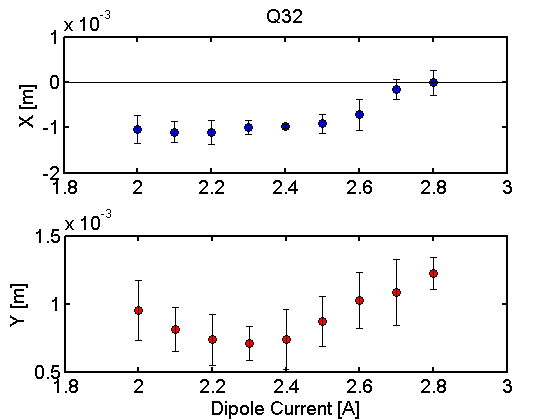
\includegraphics[width=0.45\textwidth]{4.figures/ring_steering_D15_it2_Q32.png}}
\hspace{.05in}
\subfloat[Position in focusing quad]{
	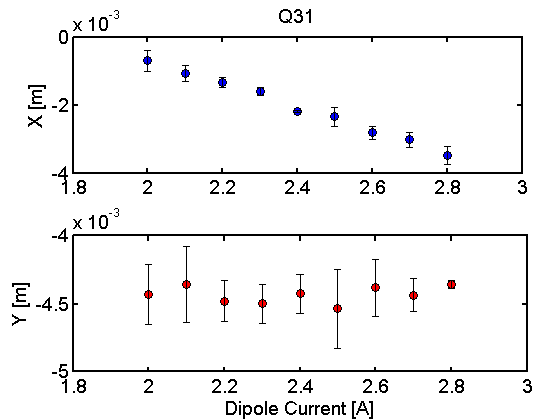
\includegraphics[width=0.45\textwidth]{4.figures/ring_steering_D15_it2_Q31.png}}
\hspace{.25in}
\raggedleft
\subfloat[RMS minimization of $x_F$ and $x_D-x_F$]{ \label{fig:ring_steering:rms}
	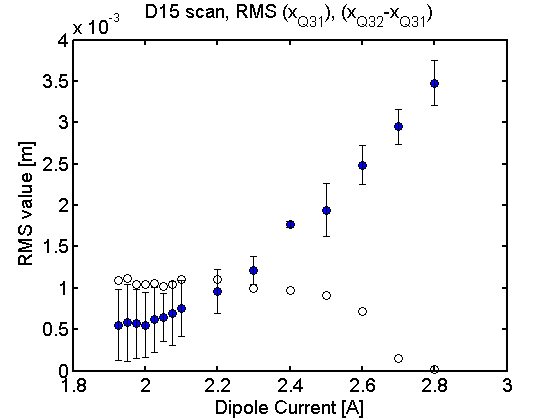
\includegraphics[width=0.45\textwidth]{4.figures/ring_steering_D15_RMS_it2.png}}

\caption{Steering through D15 using two different algorithms, 11/11/15}
\label{fig:injection_steering}
\end{figure}


\section{Points Rejection}
%%% Point rejection algorithm
A weakness of the  $\| x_D \|$ minimization is that occasionally the data will not fall on a straight line. This is most likely due to scraping between the dipole and BPM or noise in the region near the pulser. In the ring steering scripts, I have implemented a points rejection critera that throws away quad position data with errorbar $> 1$ mm. As the errors is proportional to the uncertainty in the fitted slope of the quad response, large non-linearities in the quad response will manifest as large error bars. This is typical of large centroid excursion in either the quad or the BPM.


%%%%%% closing orbit
\section{Closing the orbit}

The final step is to set the current in the dipoles near the end of the ring so that the closed orbit is close to the p1 closed orbit.  Two dipoles are required for control of x and x'. Naively, one would vary the last two dipoles, D35 and PD-Rec. Unfortunately PD-Rec has significant coupling with the first turn beam position. For a scan of PD-Rec from $8.25 \rightarrow 13.75$ A, the position of the beam in the first BPM varies in the range $\Delta x = \pm 2$mm. Changing PD-Rec would mean changing all ring dipole settings to compensate, which is undesirable. 

It is possible but difficult to optimize the value of PD-Rec. Instead, I assume that the present setting (PD-Rec I$=11$ A) is reasonably close to the ideal value such that closing the orbit with D34 and D35 will result in a bump in the closed orbit in that neighborhood. It may be possible to infer, based on the difference in the D34 currents optimized for a) steering through RQ69 and RQ70 and b) a closed orbit solution, the size of the orbit bump. 

To set D34 and D35, I scan the currents in each and record the BPM response for the first four turns in the first 3 BPMs. I try to minimize the RMS change in position between turn 1 and turn $N\le4$ in the first three BPM's. For each BPM 1-3, I define an RMS quantity $\sqrt{\frac{1}{3}\left[ \left(x_2-x_1\right)^2+\left(x_3-x_1\right)^2+\left(x_4-x_1\right)^2\right]}$. In order to find a good closed orbit, I ran 3 scans, increasing the resolution and/or re-centering the scan range for each successive scan. Scan takes $\sim$13 minutes to read 3 BPMs for 11 current settings in each dipole. 

%todo: Update this plot with new data
\begin{figure}[htb]
\centering
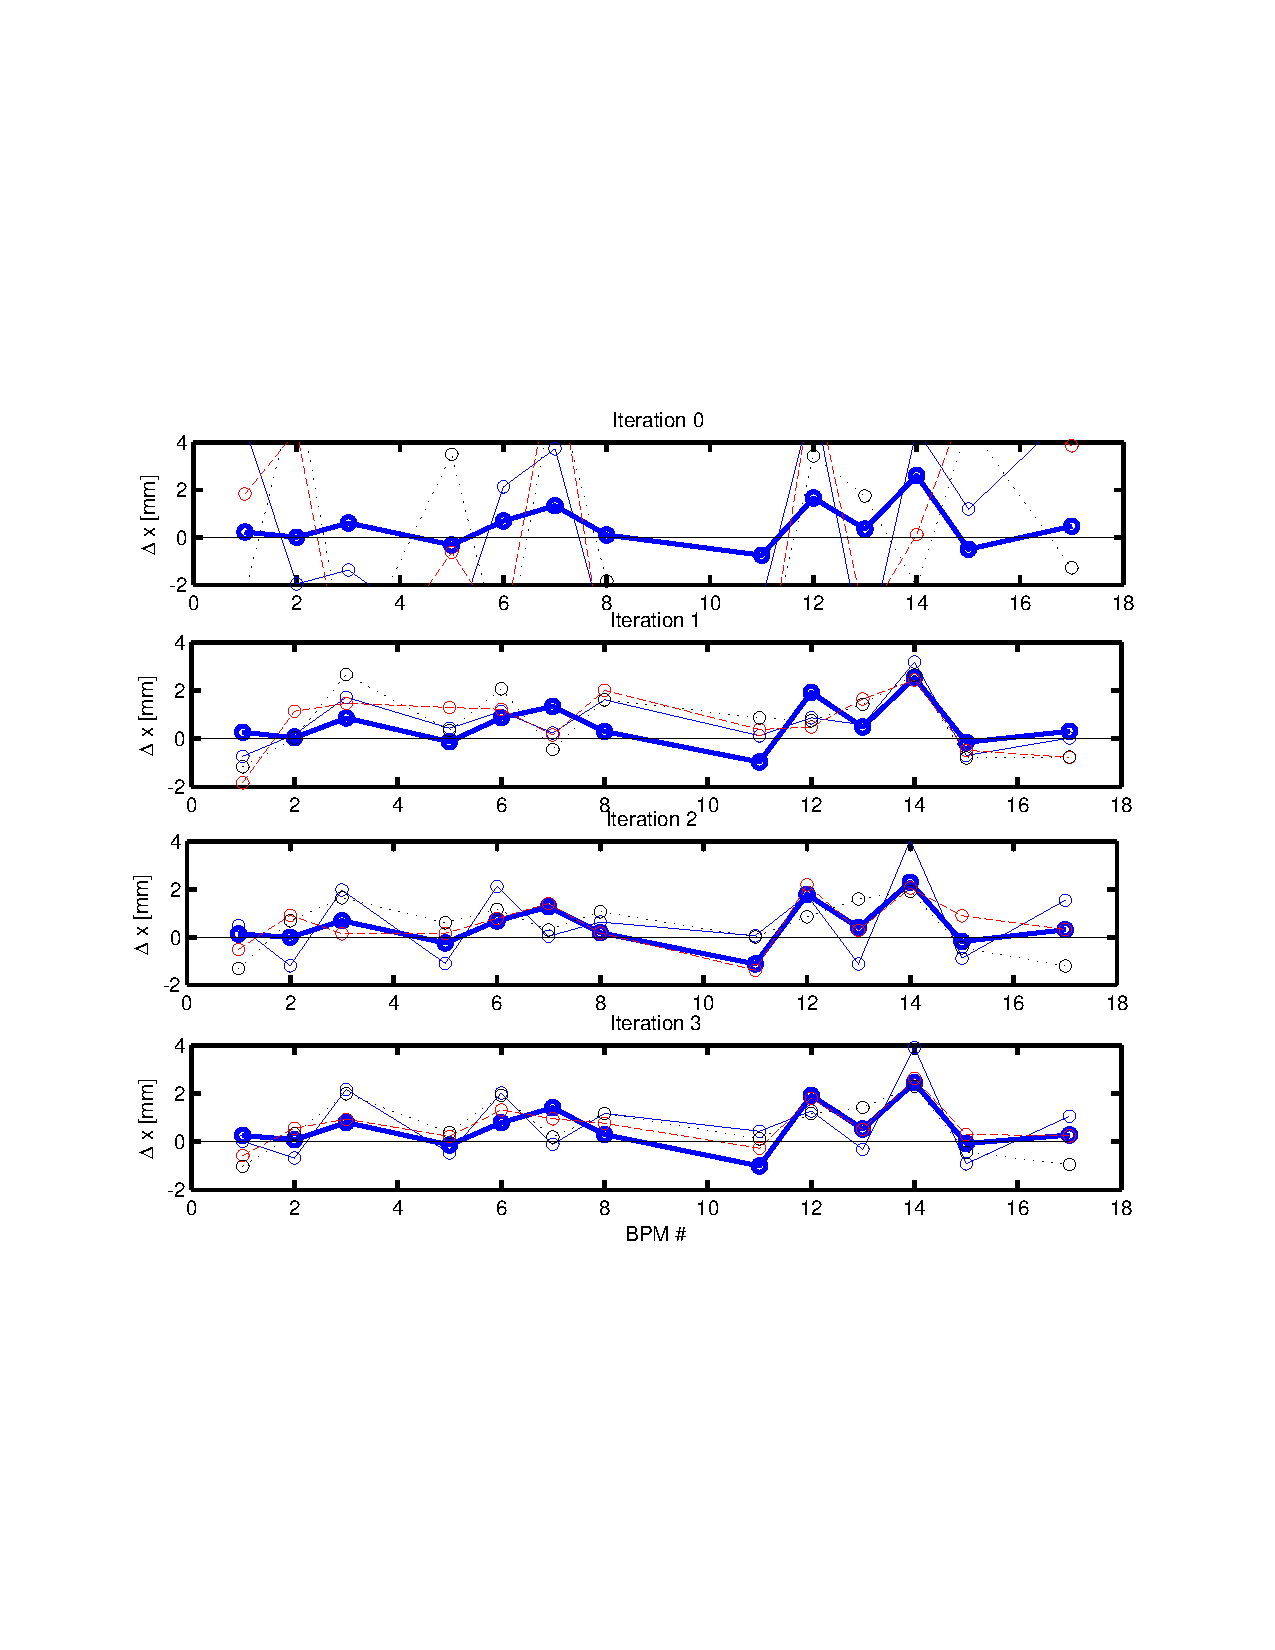
\includegraphics[width=\textwidth,trim={.5in 2.7in .5in 2.7in},clip]{4.figures/closing_orbit_BPMs.pdf}
\caption{BPM response for first 4 turns, for D34, D35 currents listed in table \ref{tab:close_ring}. 1st turn: heavy blue trace. 2nd turn: solid blue. 3rd turn: long dash red. 4th turn: short dash black.}
\label{fig:close_BPMs}
\end{figure}

\begin{figure}[htb]
\centering
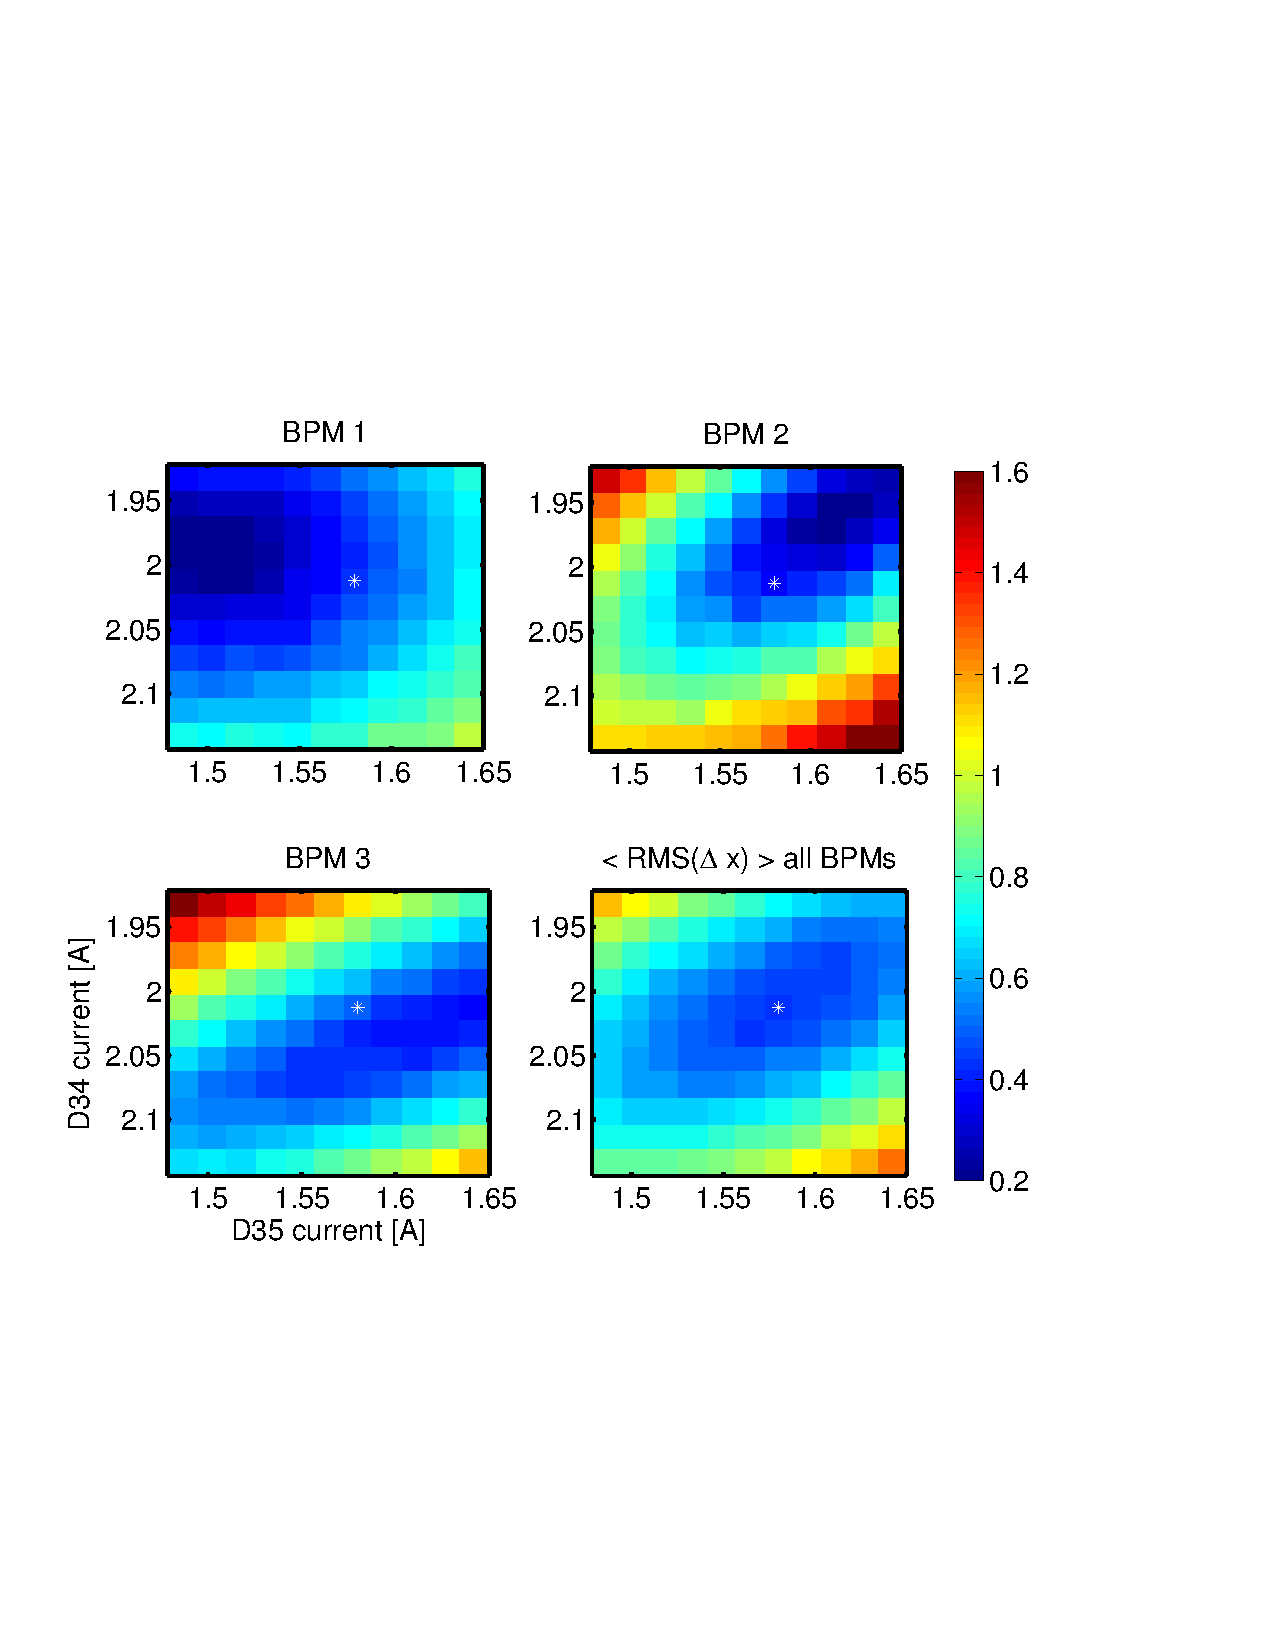
\includegraphics[width=\textwidth,trim={0 2.7in 1in 2.7in},clip]{4.figures/closing_orbit_iteration3.pdf}
\caption{Scan results for first 3 BPMs for iteration 3 in table \ref{tab:close_ring}. Color scale is rms value of $\Delta x$ over first 4 turns [mm], white asterisk indicates optimal setting (D34=2.0129 A, D35=1.5802 A) }
\label{fig:close_scan}
\end{figure}

